\subsection{Fragebogen} \label{fragebogen-1}

\todo[inline]{Verantwortlich: Boris}

Ein Fragebogen kann als Formular definiert werden, das einen Satz von Fragen enthält, die für einen bestimmten Zweck definiert wurden \cite{gault-questionnaire}.
Hier dient der Fragebogen als Befragungsinstrument für die Realisierung unseres Projekts. 
Hierfür wurden fü­r die Ausarbeitung die Hauptkomponenten definiert, die Auskunft über das Problem der Studie und über die Versuchsperson geben. \\

Für das erste Experiment dieser Studie sieht das Fragebogenmodell folgendes aus: eine Liste von elf Emotionen (Angst, Aufregung, Frustration, Langeweile, Neugier, Ruhe, Traurigkeit, Überraschung, Wut, Befriedigung und Nervosität) mit je vier nummerierten  Check-Boxen, die nach der Intensität des Gefühls der betreffenden Emotion angekreuzt werden sollten. 
Das erste Feld entspricht der niedrigsten Intensität und das vierte Feld der höchsten Intensität. Man hat auch die Möglichkeit, keine Check-Box auf eine Emotion anzukreuzen, wenn man seiner Meinung nach die Emotion gar nicht gespürt hat. 
Das würde dem Intensität Null entsprechen. Zudem soll man auch für jedes Viertel der Zeit eines Szenario die dominante Emotion wählen. \\


\begin{figure}[H] \centering
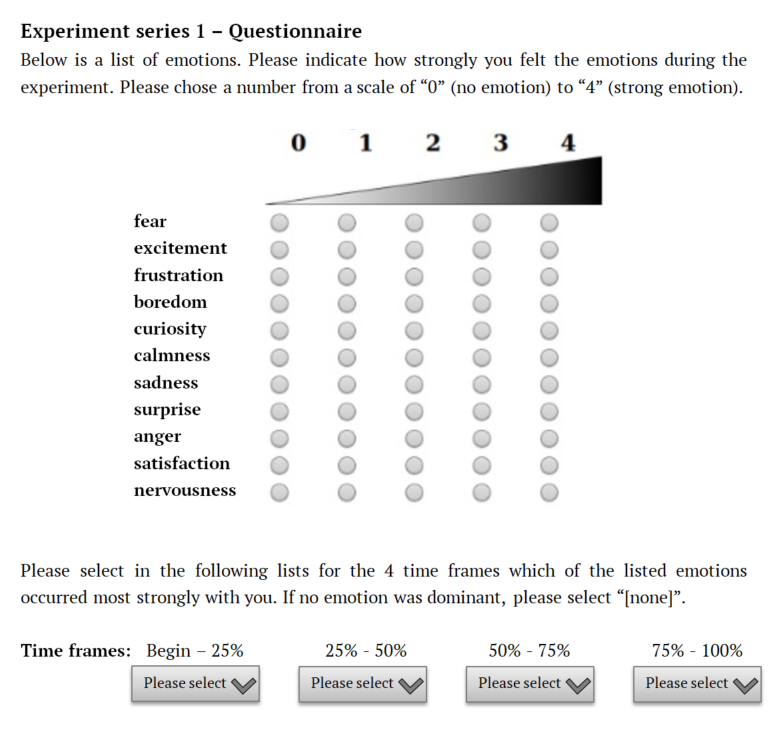
\includegraphics[width=\textwidth]{Images/questionnaire-1.png} 
\vspace{-0.3cm} 
\caption{Bild des verwendeten Fragebogens.}
\label{fig-questionare-1} 
\end{figure}

